%\section{Un Peu d'Histoire}

\subsection{Préhistoire et Antiquité}

\begin{frame} \frametitle{Préhistoire et Antiquité}
  \begin{itemize}
  \item Préhistoire : Observation et reproduction de phénomènes
    (alignement de Carnac). Notion de cycles et donc de règles (que
    l'on doit pouvoir utiliser).


  \item Antiquité : L'étude du comportement de la matière est une des
    branches de la philosophie. Début de la méthode expérimentale
    (médecine).

  \item 700 Av JC apparition des mathématiques (lat. \emph{mathema}:
    savoir, connaissance, compréhension, perception)
    \note[item]{l'étude des mathématiques a commencé en se posant des questions sur le monde}

  \item 600 av. JC : Démocrite, Thalès : «~le monde peut être compris
    comme le résultat de processus naturels~» (et non comme l'action
    des dieux).  Début des vérifications expérimentales avec Archimède
    et Eratosthène.

    \note[item]{C'est Thales qui serait le créateur de la géométrie
      Grec et c'est cette géométrie(mesure de la terre) en tant que
      théorie mathématique abstraite(plutôt qu'une collection de faits
      empiriques) supportée par des preuves déductives rigoureuses qui
      a été un des moments critiques de la pensée scientifique}

  \end{itemize}

\end{frame}
\subsection[Moyen Age-19ème]{Du Moyen Age au 19ème Siècle}
\begin{frame} \frametitle{Du Moyen Age au 19ème Siècle}
  \begin{itemize}
  \item Moyen Age : progrès scientifiques dûs aux Arabes et aux Indiens et mise en
    place d'outils mathématiques (arithmétique, algèbre, algorithmique).

  \item XIIe siècle : apparition du mot «physique» pour désigner la
    science de la nature.

  \item XVIe siècle : Tycho-Brahé (observations
    astronomiques). Copernic. Kepler (mouvements des planètes).

    \note[item]{L'astrophysique a été un des sujets les plus
      étudiés, qui a stimulée beaucoup de travaux, déjà au temps des
      greac, Platon proposa le sujet suivant à ces ``étudiants'' :
      \emph{expliquer le mouvement des corps célestes par une théorie
        géométrique}}

  \item XVIIe siècle : Galilée 1er physicien dans le sens actuel
    (s'appuie sur les mathématiques pour décrire le monde) et 1er
    vulgarisateur (entre autres). Descartes (raisonnement,
    déduction). Pascal. Newton (mécanique classique,
    gravitation). Leibniz (calcul infinitésimal, énergie, loi de
    conservation, dualité onde-corpuscule).

    \note[item]{c'est Newton qui conceptualisa la force par un
      vecteur(\emph{Principia}), bien qu'il ne donna pas de définition
      formelle, c'est William Rowan Hamilton qui le fit un siècle et
      demi après \emph{Principia}}


  \end{itemize}

\alert{La physique devient la science qui étudie les phénomènes
  matériels et qui établit les lois qui les régissent.}

\end{frame}

\subsection[20ème -- ...]{Début du 20ème Siècle à nos jours}
\begin{frame} \frametitle{Début du 20ème Siècle à nos jours}
  \begin{itemize}
  \item Ère industrielle : thermodynamique, machine à vapeur
    (Carnot). Unification de l'électricité et du magnétisme. Équations
    de Maxwell.

    \note[item]{Maxwell, James (1831-1879), Scottish mathematician and
      physicist who published physical and mathematical theories of
      the electromagnetic field.  Maxwell's formulation of electricity
      and magnetism was published in A Treatise on Electricity and
      Magnetism (1873), which included the formulas today known as the
      Maxwell equations. Maxwell also showed that these equation
      implicitly required the existence of electromagnetic waves
      traveling at the speed of light. He also proposed a physical
      theory of ether. He abandoned attempts to formulate a specific
      mechanical model, instead using the formalism of Lagrangian
      mechanics. }

  \item Époque moderne : radioactivité (Becquerel). Existence du photon
    (Einstein, Planck). Relativité (Einstein,
    Poincaré). Electrodynamique quantique (Feynman), magnétisme
    (Néel),Mécanique quantique, mécanique des ondes (E. Schrödinger)...

    \note[item]{Schrödinger, Erwin (1887-1961), Austrian physicist who
      invented wave mechanics in 1926. Wave mechanics was an
      independent formulation of quantum mechanics to Heisenberg's
      matrix mechanics. Like matrix mechanics, wave mechanics
      mathematically described the behavior of electrons and
      atoms. The central equation of wave mechanics, now known as the
      Schrödinger equation, turned out to be much simpler for
      physicists to solve in most cases.}

  \end{itemize}

  \begin{alertblock}{Mathématiques}
    Les Mathématiques sont sous jacentes à tous ces développements.
  \end{alertblock}

\end{frame}

\begin{frame}
  \frametitle{Encore un peu d'histoire}

  \begin{block}{Newton, Isaac (1642-1727) }
    \begin{columns}[c]
      \begin{column}{.3\textwidth}
        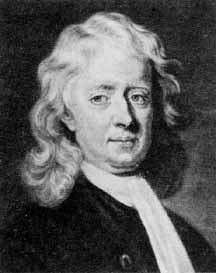
\includegraphics[height=.25\textheight]{Figures/photos/Newton}
      \end{column}
      \begin{column}{.55\textwidth}
        All in nature reduces to differential equations
      \end{column}
    \end{columns}

  \end{block}

  \begin{block}{Planck, Max (1858-1947)}
    \begin{columns}[c]
      \begin{column}{.3\textwidth}
        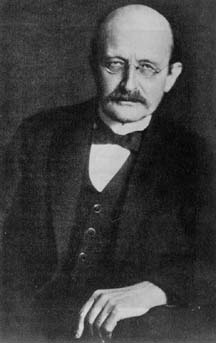
\includegraphics[height=.25\textheight]{Figures/photos/Planck}
      \end{column}
      \begin{column}{.55\textwidth}
        ...Present day physics, as far as it is theoritically organized,
        is completely governed by a system of space-time differential
        equations.
      \end{column}
    \end{columns}
  \end{block}
 \end{frame}
